\scanpage{13}
\mspage{3}

forme initiale (cas $\alpha,\beta$) implique Hyp. 2 sous sa forme générale (en termes de $\alpha_0,\alpha_1,\ldots\alpha_n$).

\uline{Hyp.} 2': Pour tout $\alpha_0\in\mathrm{Ob}\,A$, le foncteur induit $A_{/\alpha_0}\unsure{\xrightarrow{\varphi}|\twoheadrightarrow|\longrightarrow}\mathcal X_{/\alpha_0}$ satisfait \unsure{à|:} Hyp 2 i.e. pour tout diagramme
\diagram{\begin{tikzcd}[ampersand replacement=\&,column sep=small,row sep=small]
\alpha_1\arrow[dr]\&\&\alpha_2\arrow[dl]\\
\&\alpha_0\&
\end{tikzcd}}
, regardant les carrés commutatifs dans $A$ qui le complètent en
\diagram{\begin{tikzcd}[ampersand replacement=\&,column sep=small,row sep=small]
\&\gamma\arrow[dl]\arrow[dr]\&\\
\alpha_1\arrow[dr]\&\&\alpha_2\arrow[dl]\\
\&\alpha_0\&
\end{tikzcd}}
, i.e. les objets de $A_{/\alpha_1\times_{\alpha_0}\alpha_2}$, la famille des flèches correspondantes
\[U_\gamma\longrightarrow U_{\alpha_1}\times_{U_{\alpha_0}}U_{\alpha_2}\]
est couvrante (i.e., épimorphique).

Les hypothèses Hyp 1, 2, 2' se reformulent joliment, en termes du prolongement canonique
\[\varphi_!:\widehat A\longrightarrow\mathcal X\]
de $\varphi$ en un foncteur 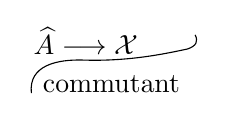
\begin{tikzpicture}[baseline=(w.base)]
\node[anchor=west,inner sep=0pt] (w) at (0,0) {commutant};
\node[anchor=west,inner sep=0pt] at (-.12,.54) {\inserted{$\widehat A\longrightarrow\mathcal X$}};
\draw (-.14,-.12)..controls(-.18,.24)and(.2,.31)..(.52,.3)..controls(1.12,.28)and(1.6,.39)..(1.84,.44)..controls(1.96,.48)and(1.98,.54)..(1.94,.62);
\end{tikzpicture} \deleted{\unsure{à|et}} aux petites $\lim_{\longrightarrow}$. Ce sont respectivement
\margin{12}
